Sana \termi{prosentti}{prosentti} tulee latinan kielen ilmaisusta \termi{pro centum}{pro centum}, joka tarkoittaa kirjaimellisesti sataa kohden tai sadasta. Prosentit ovat siis sadasosia, ja kyseessä on rationaalilukujen sovellus -- prosentteja käytetään ilmaisemaan suhteellista osuutta. Prosentin symboli on \%. Prosentin sukulaiskäsite on \termi{promille}{promille}, joka tulee vastaavasta latinan ilmaisusta \termi{pro mille}{pro mille}. Promillen symboli on \permil.

\laatikko[Prosentti ja promille]{$1$ \text{prosentti}$=1\,\% = \frac{1}{100} = 0,01$\\
$1$ \text{promille}$=1\,\permil=\frac{1}{1\,000}=0,001$}

\begin{esimerkki}
\alakohdat{
§ $0,03=\frac{3}{100}=3\,\%=30\,\permil$
§ $0,00478=\frac{0,478}{100}=0,478\,\%=4,78\,\permil$
§ $0,76=\frac{76}{100}=76\,\%=760\,\permil$
§ $1,23=\frac{123}{100}=123\,\%=1\,230\,\permil$
§ $2,10=\frac{210}{100}=210\,\%=2\,100\,\permil$
}
\end{esimerkki}

Erityisesti kannattaa huomata, että $100\,\%=1$.

%Jos sadaosien lukeminen suoraan desimaaleista tuntuu haastavalta, saadaan prosentit ''näkyviin'' kertomalla desimaaliluku sadalla. Tällöin sadasosat siirtyvät luvussa ykkösten paikalle. Tämä on kuitenkin vain matemaattinen kikka vastauksen ulkoasun muuttamiseksi -- ei välttämätöntä tehtävän ratkaisun kannalta.
%
%\begin{esimerkki}
%Esittääksemme desimaaliluku $0,017$ prosentteina, luvun voi kertoa sadalla, jolloin saadaan $100\cdot 0,017=1,7$. Siis $0,017=1,7\,\%$.
%\end{esimerkki}
%suhteellinen/absoluuttinen-tarkastelu tähän vai rationaalilukujen sovelluksiin?? esimerkkinä punapaidat 25/239 ja kultapaidat 10/55! määrässä voittaa,suhteessa häviää! :) esimerkissä myös merkkaa elävien ja kuolleiden suhdetta (piirakkadiagrammi)

Prosenttilaskennan käytännön kysymyksenasettelut ja tehtävät voidaan jakaa karkeasti neljään ryhmään. Tehtävänantojen peruskysymykset liittyvät toisiinsa seuraavalla sivulla olevan kaavion mukaisesti, missä $a$, $b$ ja $p$ ovat (mielivaltaisia) lukuja. Toisessa kaaviossa on esitetty samat kysymykset formalisoituina.
\newpage
\laatikko[Prosenttilaskennan tehtävätyypit]{
\begin{tabular}{|ccc|}
\hline 
 & & \\
\vtop{\hbox{\strut ''Kuinka monta prosenttia ($p$)}\hbox{\strut luku $a$ on $b$:stä?''}}  & $\rightleftarrows$ & \vtop{\hbox{\strut ''Kuinka paljon ($a$) on}\hbox{\strut $p$\,\% luvusta $b$?''}}\\ 
$\downarrow$ &  & $\downarrow$ \\ 
\vtop{\hbox{\strut ''Kuinka monta prosenttia ($p$)}\hbox{\strut luku $a$ on suurempi/pienempi kuin $b$?''}} & $\rightleftarrows$ & \vtop{\hbox{\strut ''Mitä ($a$) saadaan, kun $b$}\hbox{\strut kasvaa/vähenee $p$ prosenttia?''}}  \\ 
& & \\
\hline
 & & \\
\vtop{\hbox{\strut $\dfrac{a}{b}=p\,\%$}}  & $\rightleftarrows$ & \vtop{\hbox{\strut $p\,\%\cdot b=a $}}\\ 
$\downarrow$ &  & $\downarrow$ \\ 
\vtop{\hbox{\strut $\dfrac{a-b}{b}=p\,\%$}} & $\rightleftarrows$ & \vtop{\hbox{\strut $\left(1\pm p\,\% \right)b=a$}}\\ 
 & &\\
\hline 
\end{tabular}
}

Ongelmat, joiden välillä on nuoli molempiin suuntiin, ovat matemaattisesti yhtäläisiä eli ekvivalentteja. Ne voidaan esittää ja käsitellä molemmin tavoin, vaikka ratkotaankin edelleen samaa ongelmaa. Ylärivin kaksi tapausta ovat yksinkertaisimmat tehtävänannot, ja ne käsitellään ensin. Alarivin kysymyksenasetteluiden formalisointi (lausekkeiksi ja yhtälöksi kirjoittaminen) vaatii ylärivin kysymysten tekniikkaa. (Kaavion jäsentely tukee myös kuitenkin sitä, että ensin voitaisiin opetella vasemmalla puolella olevat ja sen jälkeen erillisesti oikealla puolella olevat tehtävätyypit -- tai toisinpäin.)

Tehtävien ratkaisu saattaa vaatia edellä mainittujen tilanteiden yhdistelemistä ja tuntemattoman ratkaisemista yhtälöstä. Erilaisten suhteiden prosentuaalisille ilmaisuille on vakiintunut omat nimensä, jotka kannattaa opetella.

\laatikko[Vertailuprosentti ja perusarvo]{
    \termi{vertailuprosentti}{Vertailuprosentilla} tarkoitetaan sitä, kuinka paljon jokin on jostakin, mihin verrataan.
    Lukua, johon verrataan tai jota muutetaan, kutsutaan \termi{perusarvo}{perusarvoksi}.}

Vertailuprosentilla vastataan siis kysymykseen ''kuinka monta prosenttia luku $a$ on luvusta $b$?'', ja vertailuprosentti saadaan laskutoimituksesta $\frac{a}{b}$, joka tulkitaan lopullista vastausta varten prosentteina eli sadaosina. Koska jakolasku ei ole vaihdannainen, on tärkeää varmistaa, että tehtävässä suhde muodostetaan oikein päin. Suhdetta muodostettaessa se, mihin verrataan, toimii jakajana.

\begin{esimerkki}
Kuinka monta prosenttia
\alakohdat{
§ luku $20$ on luvusta $80$?
§ luku $80$ on luvusta $20$?
}
	\begin{esimratk}
	\alakohdat{
	§ Perusarvo on tässä tapauksessa $80$ -- siihen verrataan. Lasketaan osamäärä $\frac{20}{80}$ ja esitetään vastaus prosentteina:
	$$\frac{20}{80}=\frac{2}{8}=\frac{1}{4}=0,25=25\,\%$$
	§ Nyt perusarvo on $20$, ja siihen verrataan. Lasketaan osamäärä $\frac{80}{20}$ ja esitetään vastaus prosentteina:
	$$\frac{80}{20}=\frac{8}{2}=4=400\,\%$$
	}
	\end{esimratk}
\end{esimerkki}

%Vertailuprosentti voidaan laskea paljaiden lukujen suureista äytä, että pitää olla samaa suuretta, yksiköt kyllä supistuvat pois
%ideaaliesimerkkiketju: luvuilla -> symboleilla yleisemmin -> sanallinen sovellus
%esitä todistus, mikä yhdistää kaavion alarivin jäsenet
%esimerkkiin negatiivisia lukuja jan
%pointtina nyt se, että yhtälöt ja sitten, että voidaan käsitelläkummalla tavalla tahansa
%komplementtiesimerkki tyyliin "40 kansasta vastustaa...." -> "60 prosentita kansasta ei vastusta"
% esimerkki absoluuttisesta ja suhteellisesta kasvusta, esim- yhdsityksen jäsenmäärä ja sittnen kehuskellaan... mutta pineinllä absoluuttisilla määrillä tulee hlepomin nuo isot suhteelliset :)
% KIRKOSTAEROAMISTILASTOT!!!! -> näissä kunnissa...
% kaksi esimerkkiä liuossekoituksista, kuivauksesta yms.

\begin{esimerkki}
Tarmo leikkaa pizzan neljään osaan ja syö näistä kolme.
\alakohdat{
§ Kuinka monta prosenttia pizzasta Tarmo syö?
§ Kuinka monta prosenttia pizzasta jää jäljelle?
}
	\begin{esimratk}
\alakohdat{
§ Tarmo syö $3$ palaa neljästä eli $\frac{3}{4} = 0,75$. Tämä voidaan muuttaa prosenttiluvuksi ilmaisemalla luku sadasosina.  $0,75 \cdot 100 = 75$. Siis $0,75=75\,\%$, ja Tarmo söi $75\,\%$ pizzasta.
§ Koko pizzasta otetaan pois Tarmon syömä osa jolloin jäljelle jää $100\,\% - 75\,\% = 25\,\%$. Samaan vastaukseen olisi päädytty, jos olisi muunnettu jäljellä olevien pitsapalojen määrän suhdetta koko pitsaan esittävä rationaaliluku $\frac{1}{4}$ prosenteiksi.
}
	\end{esimratk}
	\begin{esimvast}
	\alakohdat{
	§ $75$\,\%
	§ $25$\,\%
	}
	\end{esimvast}
\end{esimerkki}

\begin{esimerkki}
Alex ansaitsee kuukaudessa $3\,200$ euroa ja Antero $2\,300$ euroa.
\alakohdat{
§ Kuinka monta prosenttia Anteron tulot ovat Alexin tuloista?
§ Kuinka monta prosenttia Alexin tulot ovat Anteron tuloista?
}
 
	\begin{esimratk}
	\alakohdat{
	§ Lasketaan vertailuprosentti. Perusarvo on tehtävänannon mukaisesti Alexin palkka eli $3\,200$ euroa.
    $$\frac{2\,300}{3\,200}=0,71875\approx 0,72= 72\,\%$$
    § Lasketaan vertailuprosentti, mutta nyt perusarvona toimiikin Anteron palkka:
    $$\frac{3\,200}{2\,300}\approx1,39=139\,\%$$
    }
    \end{esimratk}
    \begin{esimvast}
    	\alakohdat{
    	§ Anteron tulot ovat $72\,\%$ Alexin tuloista.
    	§ Alexin tulot ovat $139\,\%$ Anteron tuloista.
    	}
  \end{esimvast}
\end{esimerkki}

Tapaus ''kuinka paljon on $p$\,\% luvusta $a$'' lasketaan kertolaskuna aivan niin kuin aiemmin on tehty kaikilla rationaaliluvuilla muutenkin.

\begin{esimerkki}
\alakohdat{
§ Jos luku $a$ halutaan kaksinkertaistaa, kerrotaan se kahdella: $2a$.
§ Jos käsitellään luvusta $x$ vain kolmasosaa, kerrotaan se $\frac{1}{3}$:lla: $\frac{1}{3}x$.
§ Jos halutaan tietää, mitä on kymmenen prosenttia luvusta $120$, kerrotaan se $10\,\%$:lla: $10\,\%\cdot 120=0,10\cdot 120=12$.
§ $2\,\permil$ luvusta $h$ on $2\,\permil h=0,002h$.
}
\end{esimerkki}

%\begin{esimerkki}
%alennetaan prosentuaalisesti.... kuinka monta euroa tjsp. aleni? Mikä on uusi?
%\end{esimerkki}

Joskus useita kertolaskuja täytyy ketjuttaa.

%esim. Ohut pilvipeite päästää läpi 90 % UV-säteilystä, ja varjossa oleskelu vain puolittaa aurinkoannoksen. laske kokonaisosuus
% kuinka suuri osa väestöstä... jotainsellaiast.

Usein perusarvoa ei tunneta, vaan se joudutaan ratkaisemaan yhtälöstä.

%pidä aina selvänä, ''p prosenttia... MISTÄ? Prosentteja ei käytetät yksinään, vaan ne ovat aina riippuvaisia jostain absoluuttisesta suureesta''

\begin{esimerkki}
Lennonjohtajakoulutukseen Suomessa syksllä 2014 pääsi vain kahdeksan henkilöä. Lehtiotsikoiden mukaan sisäänpääsyprosentti oli $0,67\,\%$. Kuinka monta hakijaa koulutukseen pyrki kaiken kaikkiaan? Huomio vastaustarkkuus. %Kuinka monta hakijaa koulutukseen korkeintaan pystyi olemaan, kun otetaan huomioon lähtötietojen tarkkuus?
	\begin{esimratk}
	Sisäänpääsyprosentti tarkoittaa koulutukseen päässeiden määrän suhdetta kaikkien hakijoiden määrään. Merkataan kaikkien hakijoiden määrää $y$:llä. Saadaan yhtälö $\frac{8}{y}=0,67\,\%$.
	\begin{align*}
	\frac{8}{y}&=0,67\,\% &&|\cdot y\text{ ja } (y\neq 0) \\
	8&=0,67\,\%\cdot y && \\
	8&= 0,0067y && |:0,0067 \\
	\frac{8}{0,0067}&=y && \\
	y&=\frac{8}{0,0067} && \\
	y&\approx 1\,194 \approx 1\,200
	\end{align*}
	Koska lähtötiedoilla ei tarkaksi vastaukseksi saatu luonnollista lukua (joka voisi olla hakijoiden lukumäärä), on mainostettu sisäänpääsyprosentti luultavasti pyöristetty. Koska se annetaan merkitsevän numeron tarkkuudella, annetaan myös vastaus kahden merkitsevän numeron tarkkuudella. %Hakijoita saattoi olla jotain väliltä $1\,150 -- 1\,249$.
	\end{esimratk}
\end{esimerkki}

\begin{esimerkki}
Arvonlisävero on on valtiolle perittävä vero, jota maksetaan tuotteista ja palveluista. Arvonlisäverokanta määräytyy tuotteen tyypin mukaan, ja itse veron suuruus (euroina) lasketaan osuutena tuotteen verottomasta hinnasta. Vuonna 2012 yleinen arvonlisävero oli $23$\,\% tuotteen verottomasta hinnasta.
\alakohdat{
§ Kuinka suuri arvonlisävero (euroina) maksetaan tuotteesta, jonka veroton hinta on $8,45$ euroa?
§ Kuinka suuri on tällöin verollinen eli lopullinen kuluttajahinta?
§ Kuinka monta prosenttia arvonlisä on tuotteen verollisesta hinnasta?
}
	\begin{esimratk}
	\alakohdat{
	§ Merkitään arvonlisäveron määrää (euroina) $x$:llä. Tällöin tehtävänannon ja arvonlisäveron määritelmän perusteella pätee yhtälö $\frac{x}{8,45\,€}=23\,\%$. Muuttamalla prosenttiluku desimaalimuotoon (laskimen käytön helpottamiseksi) ja kertomalla yhtälön molemmat puolet nimittäjällä saadaan ratkaisuksi $x=0,23\cdot 8,45\,€=1,9435\,€\approx 1,90\,€$.
	§ Koska veroton hinta on $8,45$ euroa, ja tämän lisäksi maksetaan arvonlisäveroa $1,90$ euroa, saadaan lopulliseksi myyntihinnaksi $8,45\,€+1,90\,€=10,35\,€$.
	§ Verrataan arvonlisäveroa lopulliseen hintaan: $\frac{1,90\,€}{10,35\,€}\approx 0,184=18,4\,\%$. (Huomaa, että kyseinen $23\,\%$:n arvonlisävero \textit{ei} siis tarkoita, että $23\,\%$ tuotteen myyntihinnasta on veroa!)
	}
	\end{esimratk}
	\begin{esimvast}
	\alakohdat{
	§ $1,90\,€$
	§ $10,35\,€$
	§ $18,4\,€$
	}
	\end{esimvast}
\end{esimerkki}

%\begin{esimerkki}
%Vuonna 2000 täysi-ikäisiä Suomen kansalaisia oli..., joista Väestörekisterikeskuksen tietojen mukaan .... oli naisia ja ... miehiä. Kansanterveystilastoista käy ilmi, että jyseisenä vuonna $5,6$\,\% aikuisista miehistä ja $3,4$\,\% aikuisista naisista oli käyttänyt elinaikanaan lääkkeitä päihdetarkoituksessa. Kuinka monta prosenttia aikuisista kaiken kaikkiaan oli käyttänyt elinaikanaan lääkkeitä päihdetarkoituksessa vuonna 2000?
%	\begin{esimratk}
%	
%	\end{esimratk}
%	\begin{esimvast}
%		$4,5$\,\% aikuisista.
%		\end{esimvast}
%\end{esimerkki}

%TAPA 1, TAPA 2 jne.

\begin{esimerkki}
Psykoosilääke olantsapiinin yleinen haittavaikutus on painonnousu: yhdellä kolmasosalla käyttäjistä paino (massa) nousee kuuden ensimmäisen viikon aikana noin seitsemän prosenttia, yhteensä keskimäärin $5,5$ kilogrammaa. Mikä on tällaisen kolmannekseen kuuluvan keskimääräisen henkilön massa painonnousun jälkeen?
	\begin{esimratk}
Voimme merkata alkuperäistä painoa (massaa) kilogrammoissa $x$:llä. Tehtävänannon perusteella $5,5$ kilogramman absoluuttinen kasvu vastaa $7$\,\%:n suhteellista kasvua. Tästä saadaan yhtälö $5,5\,$kg$=0,07x$, jonka ratkaisuna saadaan $x=\frac{5,5\,\textrm{kg}}{0,07}\approx78,57$\,kg. Lopullinen vastaus saadaan, kun tähän alkuperäiseen massaan lisätään tuo mainittu $5,5$ kilogrammaa: $\frac{5,5\,\textrm{kg}}{0,07}+5,5$\,kg$\approx84,1$. (Huomaa, että tehtävänannon tietoa "yhdellä kolmasosalla" ei tarvittu ratkaisuun.)
	\end{esimratk}
    \begin{esimvast}
    Keskimääräisen henkilön massa painonnousun jälkeen on $84,1$ kilogrammaa.
    \end{esimvast}
\end{esimerkki}

%--------------- sovellukset vvvv ----------------------

%esimerkki,että jos laittaa väärinpäin, tulee negatiivista, MUTTA SE EI HAITTAA :))

\laatikko[Muutosprosentti]{
Prosentteja käytetään usein ilmaisemaan suureiden muutoksia, esimerkiksi luku $a$ kasvaa luvuksi $b$. \termi{muutosprosentti}{Muutosprosenttia} laskettaessa muutoksen suuruutta verrataan alkuperäiseen lukuun. Perusarvona on siis alkuperäinen arvo, johon nähden muutos on tapahtunut. Muutosta merkitään yleensä symbolilla $\Delta$ (kreikan kielen suuri \textit{delta}).
    
    \termi{absoluuttinen muutos}{Absoluuttinen muutos} luvusta $a$ lukuun $b$ on $b-a$.
    \termi{suhteellinen muutos}{Suhteellinen muutos} saadaan suhteuttamalla absoluuttinen muutos alkuperäiseen lukuun $a$ eli laskemalla
 \[ \Delta_{\text{suhteellinen}} = \frac{\Delta_{\text{absoluuttinen}}}{a} = \frac{b-a}{a} \]
    
Muutosprosentti saadaan suhteellisesta muutoksesta muuttamalla se prosenttiluvuksi
\[ \Delta_{\text{prosentti}} = \Delta_{\text{suhteellinen}} = \frac{b-a}{a} \] tulkittuna prosenteissa.

} %liikaa laatikkoa

\begin{esimerkki}
Vesan paino on tammikuussa $68$\,kg ja kesäkuussa $64$\,kg.
    \alakohdat{
§ Mikä on Vesan painon \textit{absoluuttinen muutos}?
§ Mikä on Vesan painon \textit{muutosprosentti} (eli suhteellinen muutos)?
}
    
	\begin{esimratk}
	\alakohdat{
§ Halutaan tietää Vesan painon \textit{absoluuttinen muutos} eli muutos kiloina tammikuusta kesäkuuhun.
    \[
       \Delta_{\text{absoluuttinen}} = b - a = 64\,\text{kg} - 68\,\text{kg} = -4\,\text{kg}
    \]

Vesan paino on muuttunut $-4$ kiloa, eli Vesa on laihtunut $4$ kiloa.

§ Halutaan tietää Vesan painon muutos \textit{prosentteina} tammikuusta kesäkuuhun.

        \[\Delta_{\text{prosentti}}
            = \frac{\Delta_{\text{absoluuttinen}}}{a}
            = \frac{-4}{68} \approx -0,06
            = -6\,\%   
        \]
    
        Vesan paino on muuttunut kuudella prosentilla negatiiviseen suuntaan, eli Vesa on laihtunut kuusi prosenttia.
   }
    \end{esimratk}
    \begin{esimvast}
    \alakohdat{

§ Vesa on laihtunut $4$ kiloa.
§ Vesa on laihtunut $6\,\%$.
 }

    \end{esimvast}
\end{esimerkki}

%virheprosentti (vaaka + jotain muuta, labra?)

\laatikko[Erotusprosentti]{
    Muutosprosentille läheinen käsite on \termi{erotusprosentti}{erotusprosentti}. Erotusprosentti ilmaisee kuinka monta prosenttia jokin on suurempi tai pienempi kuin joku toinen. Suhteellinen erotus saadaan laskemalla lukujen absoluuttinen erotus $|b-a|$ ja vertaamalla sitä perusarvoon, joka on aina kuin-sanan jälkeinen arvo.
    
Jos luku $a$ on $p\,\%$ pienempi tai suurempi luku $b$, pätee
    \[ p = \frac{|b-a|}{b}. \]
}
    
\begin{esimerkki}
Miniluumutomaatit maksavat normaalisti $4,80$ euroa kilolta. Nyt ne ovat kuitenkin alennuksessa ja maksavat $2,50$ euroa kilolta.
     \alakohdat{
        § Kuinka monta prosenttia enemmän miniluumutomaatit maksavat normaalisti kuin alennuksessa?
        § Kuinka monta prosenttia vähemmän miniluumutomaatit maksavat alennuksessa kuin normaalisti?
    }
	\begin{esimratk}

     \alakohdat{
 § Verrataan absoluuttista erotusta alennettuihin miniluumutomaatteihin:
\begin{align*}
     &\frac{|b-a|}{b}  = \frac{|2,50-4,80|}{2,50} = \frac{|-2,30|}{2,50} \\
     = &\frac{2,30}{2,50}  = 0,92 = 92,0\,\%.
\end{align*}
§ Verrataan absoluuttista erotusta normaalihintaisiin miniluumutomaatteihin:
\begin{align*}
     &\frac{|b-a|}{a} = \frac{|2,50-4,80|}{4,80} = \frac{|-2,30|}{4,80} \\
     = &\frac{2,30}{4,80}  \approx 0,479  = 47,9\,\%.
\end{align*}
	 }
\end{esimratk}		
     \begin{esimvast}
      \alakohdat{
     § Miniluumutomaatit maksavat normaalisti $92,0$\,\% enemmän kuin alennuksessa.
     § Miniluumutomaatit maksavat alennuksessa $47,9$\,\% vähemmän kuin normaalisti.
     }
     
Huomataan, että se mihin verrataan, on merkittävää ja vaikuttaa tulokseen.
      \end{esimvast}
\end{esimerkki}

Lauseella ''kaksi kertaa enemmän'' tarkoitetaan usein yleiskielessä kaksinkertaista. Matemaattisesti nämä ovat kuitenkin eri asioita. Sekaannuksen vuoksi on syytä olla käyttämättä tällaista ilmaisua. %parempaan paikkaan

\laatikko[Prosenttiyksikkö]{
\termi{prosenttiyksikkö}{Prosenttiyksikköä} käytetään mittaamaan prosenttilukujen absoluuttista muutosta. Esimerkiksi $3\,\%$ on yhden prosenttiyksikön suurempi kuin $2\,\%$, mutta $50\,\%$ suurempi kuin $2\,\%$. Jos prosenttiluku muuttuu, muutos voidaan ilmaista joko prosentteina (suhteellinen muutos) tai prosenttiyksikköinä (absoluuttinen muutos).
}

Prosentin ja prosenttiyksikön merkitysero on keskeinen esimerkiksi talousuutisten tulkinnassa.

\begin{esimerkki}
    Tuotteen markkinaosuus on vuoden tammikuussa $10$\,\% ja kesäkuussa $15$\,\%.
    \alakohdat{
    § Kuinka monta prosenttia tuotteen markkinaosuus on noussut tammikuusta kesäkuuhun?
    § Kuinka monta prosenttiyksikköä tuotteen markkinaosuus on noussut tammikuusta kesäkuuhun?
    }

    \begin{esimratk}
    \alakohdat{
    § Tuotteen markkinaosuuden muutos prosentteina:
          \[
                \frac{15-10}{10} = \frac{5}{10} = 0,5 = 50\,\%.
          \]
	§ Tuotteen markkinaosuuden muutos prosenttiyksiköinä $15\,\%-10\,\%=5\,\%$
	}
    \end{esimratk}
	\begin{esimvast}
\alakohdat{
§ $50$ prosenttia
§ $5$ prosenttiyksikköä
}
	\end{esimvast}
\end{esimerkki}

%esimerkki pulssioksimetrista prosenttiyksikköön, happisaturaatio, rajat


Kun jokin luku $a$ kasvaa $p\,\%$, täytyy laskea ensin, kuinka paljon on $p\,\%$ kyseisestä luvusta $a$ ja sitten lisätä saatu luku alkuperäiseen $a$:han. Kyseinen lauseke sievenee erittäin käyttökelpoiseen tulomuotoon:

$$a+ p\,\% \cdot a=a+ \frac{p}{100} \cdot a = (1+\frac{p}{100})a $$

Perusarvon $a$ edessä olevaa kerrointa $1+\frac{p}{100}$ sanotaan \termi{prosenttikerroin}{prosenttikertoimeksi}. Jonkin suureen tai luvun vähentyessä tietyllä prosenttimäärällä toimitaan samoin, mutta suoritetaan vähennyslasku:
$$a \mapsto (1-\frac{p}{100})a$$
On tärkeä taito, että prosenttikertoimesta osaa lukea heti, mitä perusarvolle on tehty.
%laatikko: jos prosenttikerroin on 0<x<1, niin perusarvo on pienentynyt, jos prosenttikerroin on >1, perusarvo on kasvanut

%esim., taulukoi prosentuaalisia muutoksia ja prosentitkertoimia :)

\begin{esimerkki}
Jos sadan euron hintaisen tuotteen hintaa on alennettu $25$ prosenttia, niin alennettu hinta on $75$ euroa. Jos sen sijaan alkuperäinen hinta nousee $15$ prosenttia, niin tuotteen uusi hinta on $115$ euroa. Perusarvo on molemmissa tapauksissa $100$ euroa.
    
    \begin{center}
        
\includegraphics[scale=.25]{pictures/Kuva13-1-100.pdf}
        
\includegraphics[scale=.25]{pictures/Kuva13-2-75.pdf}
        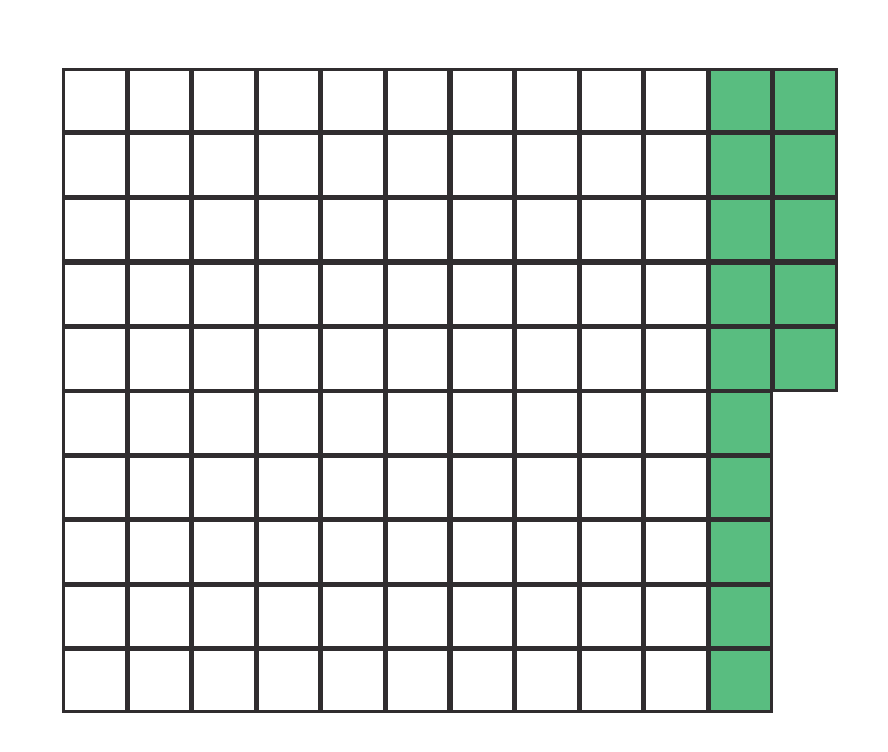
\includegraphics[scale=.25]{pictures/Kuva13-3-115.pdf}
    \end{center}
\end{esimerkki}

\begin{esimerkki}
Tuotteen hintaa korotettiin $15$\,\%, jolloin hinnaksi muodostui $175$\,euroa. Kuinka suuri oli alkuperäinen korottamaton hinta?
	\begin{esimratk}
Olkoon alkuperäinen hinta $x$\,euroa. Koska hintaa on korotettu $15$\,\%, on uusi hinta $115$\,\% alkuperäisestä eli alkuperäinen hinta $x$ on kerrottu $1,15$:llä:
\begin{align*}
	1,15x	&= 175	&	&|\, \text{Jaetaan } 1,15\text{:llä}.\\
	x	&= \frac{175}{1,15} \approx 152,17
\end{align*}
	\end{esimratk}
    \begin{esimvast}
    Tuotteen alkuperäinen hinta oli $152,17$\,euroa.
    \end{esimvast}
\end{esimerkki}

Huomaa, että edellisessä esimerkissä saatuun kertoimeen $1,15 = 115\,\%$ oltaisiin päädytty myös laskemalla $x + 0,15x = (1 + 0,15)x = 1,15x$.

%\begin{esimerkki}
%
%\end{esimerkki}

\begin{esimerkki}
Eräs kauppa myy tuotteensa $5$ prosentin alennuksella. Tämä tarkoittaa, että jokaisesta hinnasta vähennetään $\frac{5}{100}$ kertaa tuotteen hinta. Jos tuotteen alkuperäinen hinta on esimerkiksi $100$\,euroa, saadaan $5\,\%$ alennus laskettua $100$\,eurosta kertomalla $100$\,euroa $5\,\%$:lla eli viidellä sadasosalla 
\[
\frac{5}{100} \cdot 100\,\text{euroa} = 5\,\text{euroa}
\]
Alennettu hinta saadaan vähentämällä alkuperäisestä hinnasta alennus eli $100\,\text{euroa} - 5\,\text{euroa} = 95\,\text{euroa}$.

Jos tuotteen alkuperäinen hinta on $14,50$\,euroa, on alennuksen määrä
\[
	\frac{5}{100} \cdot 14,50\,\text{euroa} = 0,725\,\text{euroa}.
\]
Alennettu hinta on tällöin $(14,50 - 0,725)\,\text{euroa} \approx 13,78\,\text{euroa}$.

Samaan tulokseen pääsee vielä kätevämmin, kun ajattelee alennuksen määrän sijaan sitä, kuinka suuri osa hinnasta jää jäljelle. Jos alennus on $5\,\%$, jää hinnasta jäljelle $100\,\% - 5\,\% = 95\,\%$. Jos alkuperäinen hinta on $14,50$\,euroa, on alennettu hinta 
\[
	\frac{95}{100} \cdot 14,50\,\text{euroa} \approx 13,78\,\text{euroa}.
\]
\end{esimerkki}

%laske esimerkkinä yhteys kahden sovellustyypin välille. a-> 1,34a & (1,34a-a)/a)=0,34